\documentclass[]{beamer}

\usepackage{beamerthemesplit} 
\usepackage{movie15}
% Other themes include: beamerthemebars, beamerthemelined, 
%                       beamerthemetree, beamerthemetreebars  
\usepackage[utf8]{inputenc}
\inputencoding{utf8}
\usepackage[T2A]{fontenc}

\title[Speech and text alignment]{Analysis of knowledge requirements for speech and text alignment problem}
\author{Bartosz Kalińczuk}
\date{\today}

\begin{document}

\begin{frame}
  \titlepage
\end{frame}
\note{Talk for 15 minutes}

\section[Outline]{}

\begin{frame}
  \tableofcontents[hideallsubsections]
\end{frame}


\section{Audio model based alignment with word granularity}
\subsection{Requirements}
\begin{frame}
    \frametitle{Required knowledge}
    \begin{itemize}
        \item knowledge about alphabet and punctuation marks
        \item phoneme set
        \item limited knowledge of graphemes to phonemes conversions
        \item model parameters for each phoneme
    \end{itemize}
\end{frame}
\subsection{Outline of algorithm}
\begin{frame}
    \frametitle{Input}
    \begin{itemize}
        \item prepared audio model $\rightarrow$ for any similar language
        \item audio recording
        \item accurate text to be aligned
    \end{itemize}
\end{frame}
\begin{frame}
    \frametitle{Algorithm}
    \begin{itemize}
        \item convert text to HMM
        \begin{itemize}
            \item create dictionary with word phoneme represantation
            \item create simple language grammar from text
            \item convert above grammar to HMM using prepared phoneme models and dictionary
        \end{itemize}
        \item apply search algorithm to find best scoring HMM state sequence
        \begin{itemize}
            \item variation of Viterbi's algorithm
            \item instead of all possible states it keeps only a priority queue with best performing sequences
        \end{itemize}
    \end{itemize}
\end{frame}
\subsection{Results - English audio model}
\begin{frame}
    \frametitle{English audio model}
    \begin{itemize}
        \item "Doktor Piotr" \newline
        After \textbf{38} seconds and after \textbf{62} words it incorrectly assigned 3 seconds to word “części” and it never recovered.
        \item  “Boże Narodzenie” \newline
        It has gone wrong after \textbf{257} seconds and \textbf{503} words on word “czarownicach”.
    \end{itemize}
\end{frame}

\begin{frame}
    \frametitle{English audio model}
    The statistics for “Boże Narodzenie” however shows, that before it goes bad it actually aligns first \textbf{503} words quite nicely:
    \begin{itemize}
        \item Maximum difference (start or end): 			\textbf{0.559s}
        \item Maximum difference (start or end), if label was to short at one end: 			\textbf{0.559s}
        \item Average difference  (start or end):			\textbf{0.032s}
    \end{itemize}
\end{frame}
\begin{frame}
    \frametitle{English audio model}
    Error counts depending on time thresholds:
    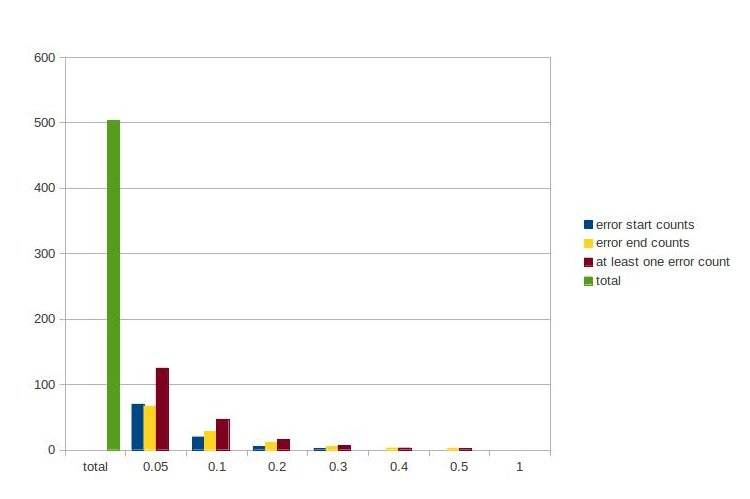
\includegraphics[scale=0.33]{boze_narodzenie_word_english_results.jpg}
\end{frame}
\subsection{Results - Russian audio model}
\begin{frame}
    \frametitle{Russian audio model - “Boże Narodzenie” statistics}
    \begin{itemize}
        \item Total number of words:				\textbf{1779}
        \item Maximum difference (start or end): 			\textbf{2.451s}
        \item Maximum difference (start or end), if label was to short at one end: 			\textbf{0.543s}
        \item Average difference  (start or end):			\textbf{0.016s}
    \end{itemize}
\end{frame}
\begin{frame}
    \frametitle{Russian audio model - “Boże Narodzenie” error counts}
    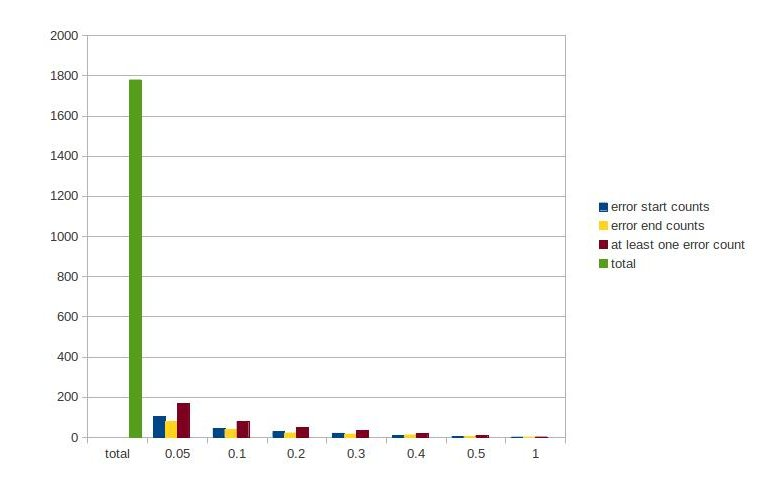
\includegraphics[scale=0.37]{boze_narodzenie_word_russian_results.jpg}
\end{frame}
\begin{frame}
    \frametitle{Russian audio model - “Doktor Piotr” sample statistics}
    \begin{itemize}
        \item Total number of words				\textbf{585}
        \item Maximum difference (start or end): 			\textbf{1.354s}
        \item Maximum difference (start or end), if label was to short at one end: 			\textbf{0.534s}
        \item Average difference  (start or end):			\textbf{0.033s}
    \end{itemize}
\end{frame}
\begin{frame}
    \frametitle{Russian audio model - “Doktor Piotr” sample error counts}
    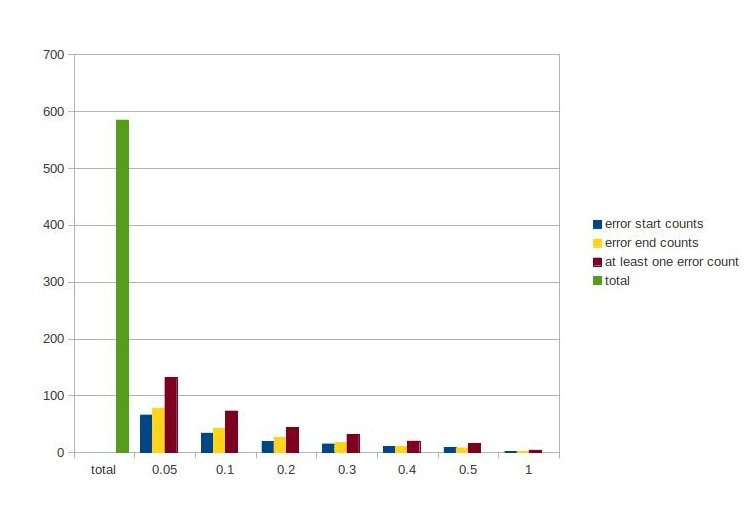
\includegraphics[scale=0.37]{doktor_piotr_word_russian_results.jpg}
\end{frame}

\section{Phoneme alignment}
\subsection{Outline of the problem}
\begin{frame}
    \frametitle{Input}
    \begin{itemize}
        \item prepared audio model $\rightarrow$ for any similar language
        \item audio recording
        \item accurate text to be aligned
        \item word alignment
    \end{itemize}
\end{frame}
\begin{frame}
    \frametitle{Problem definition}
    For each word and assigned audio part find best phoneme sequence
    \begin{itemize}
        \item each phoneme is represented with a single state
        \item state is a frame scorer
        \item state sequence is a sequential assignment of states to audio frames
        \item best state sequence is the one, that has the smallest score
        \item sequence score is the sum of scores for each frame using assigned scorer
    \end{itemize}
\end{frame}
\subsection{Using Russian phonemes models}
\begin{frame}
    \frametitle{Algorithm outline}
    \begin{itemize}
        \item in Sphinx a phoneme is modelled with a triple state HMM
        \item each state is a SenomeScorer, which calculates log likelihood of frame emission (by the state)
        \item DP algorithm calculates best state sequence
        \begin{itemize}
            \item iterates over frames
            \item partial solution is calculated for each state, where the best sequence ends with the state
        \end{itemize}
    \end{itemize}
\end{frame}
\subsection{Using trained and simplified audio model}
\begin{frame}
    \frametitle{Algorithm outline}
    \begin{itemize}
        \item EM technique applied:
        \begin{itemize}
            \item Expectation step \newline
            Alignment of phonemes given previously trained distribution
            \item Maximization step \newline
            Calculation of normal distribution for each phoneme from assigned frames
        \end{itemize}
    \end{itemize}
\end{frame}
\subsection{Results - using Russian audio model}
\begin{frame}
    \frametitle{Testing sample}
    Tests are performed using Corpora corpus, which contains audio recordings of digits, names and some unusual sentences for tens of different speakers, and all of these recordings are tagged with phonemes. \newline
    Merged recording contains a 7 minutes and 26 second of audio data, a total of \textbf{843} spoken words and \textbf{3611} phoneme labels. \newline 
\end{frame}
\begin{frame}
    \frametitle{Statistics of phoneme alignment with Russian audio model}
    The test was 
    A resulting match contained \textbf{3570} of pairs.
    \begin{itemize}
        \item Average start difference: \textbf{ 0.0571s}
        \item Average end difference: \textbf{0.0574s}
        \item Maximum time difference:\textbf{0.516s}
    \end{itemize}
\end{frame}
\begin{frame}
    \frametitle{Error counts using Russian audio model}
    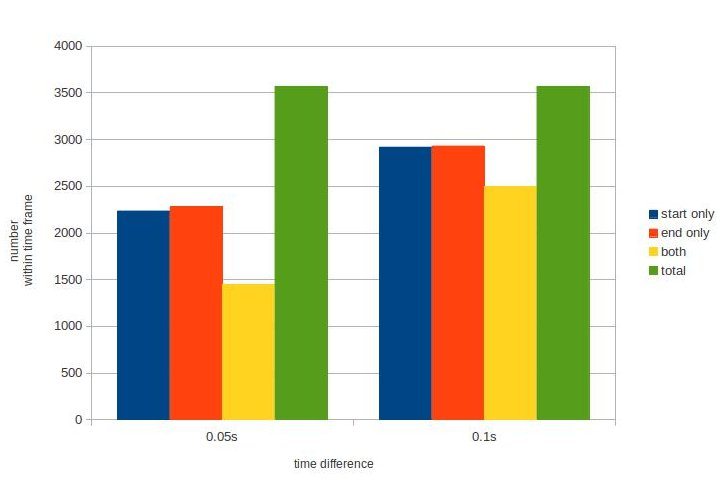
\includegraphics[scale=0.37]{corpora_phoneme_russian_counts.jpg}
\end{frame}
\begin{frame}
    \frametitle{Error counts (percentage) using Russian audio model}
    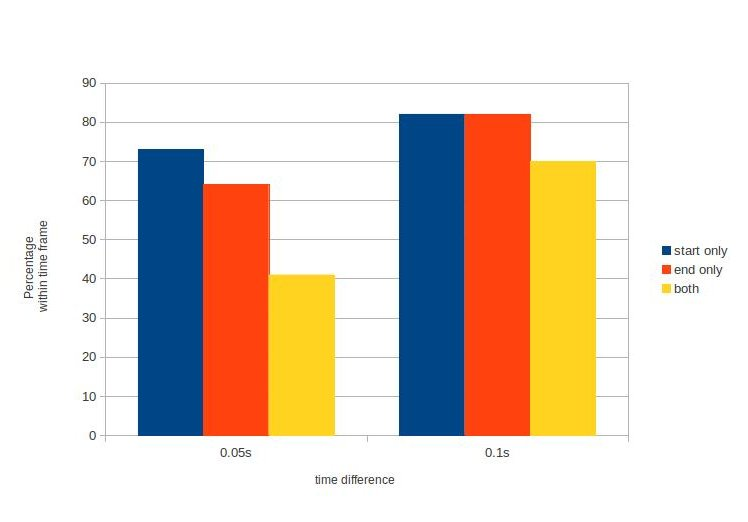
\includegraphics[scale=0.37]{corpora_phoneme_russian_results.jpg}
\end{frame}
\subsection{Results - using trained audio model}
\begin{frame}
    Matched phonemes contained \textbf{3611} pairs.
    \begin{itemize}
        \item Average start difference: \textbf{0.02402s}
        \item Average end difference: \textbf{0.02439s}
        \item Maximum time difference:\textbf{0.5131s}
    \end{itemize}
\end{frame}
\begin{frame}
    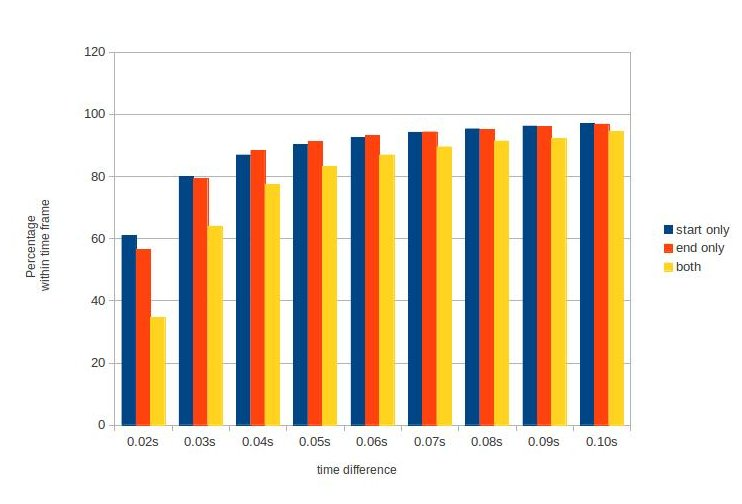
\includegraphics[scale=0.37]{corpora_phoneme_trained_results.jpg}
\end{frame}
\begin{frame}
    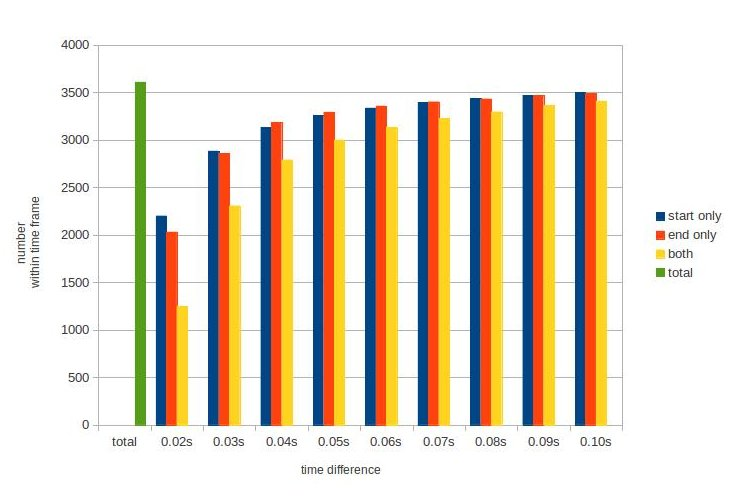
\includegraphics[scale=0.37]{corpora_phoneme_trained_counts.jpg}
\end{frame}

\section{Limited knowledge alignment}
\subsection{Requirements}
\begin{frame}
    \frametitle{Required knowledge}
    \begin{itemize}
        \item knowledge about alphabet and punctuation marks
        \item knowledge about speech frequency range and subjective perception
        \item phoneme set \footnotemark[1]
        \item limited knowledge of graphemes to phonemes conversions \footnotemark[1]
    \end{itemize}
    \footnotetext[1]{not really needed}
\end{frame}
\subsection{Pause/length based alignment}
\begin{frame}
    \begin{itemize}
        \item detect pauses/speech parts
        \item split text to parts by punctuation marks
        \item calculate expected time of each text part
        \item match speech and text parts
        \begin{itemize}
            \item sum of time differences should be minimized
            \item parts are matched sequentially
            \item DP algorithm solves this problem
        \end{itemize}
    \end{itemize}
\end{frame}
\begin{frame}
    \begin{itemize}
        \item time differences:
        \begin{itemize}
            \item there were \textbf{370} chunks (50,7\%) which time frame were within a \textbf{0.5s} difference, 
            \item average time difference was \textbf{0.77s}
            \item standard deviation was \textbf{0.84s}
            \item maximum time difference was \textbf{11.21s}
        \end{itemize}
        \item word differences:
        \begin{itemize}
            \item \textbf{393} (53.8\%) chunks had \textbf{0} difference in words
            \item \textbf{136} (18.9\%) chunks where different by \textbf{1} word (missing or additional)
            \item \textbf{48} (6.6\%) different by \textbf{2} words
            \item \textbf{56} (7.7\%) with a difference over \textbf{5} words
        \end{itemize}
    \end{itemize}
\end{frame}
\begin{frame}
    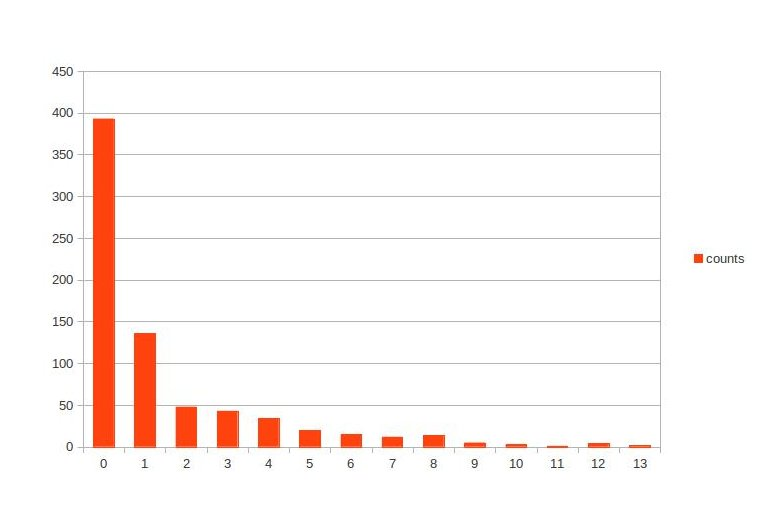
\includegraphics[scale=0.37]{length_based_results_better.jpg}
\end{frame}
\subsection{Training audio model from large chunks}
\begin{frame}
    \begin{itemize}
        \item around 54\% of the chunks were correctly identified and around another 25\% were nearly correct (less than 3 words difference)
        \item EM technique applied in similar fashion like in phoneme alignment part
        \item to improve runtime, only parts below certain threshold might be chosen
    \end{itemize}
    
\end{frame}
\subsection{Word recognition algorithm}
\begin{frame}
    \begin{itemize}
        \item merge between DP algorithm from phoneme alignment and word recognition using HMM from Sphinx library
        \item DP algorithm uses single state scorers for each phoneme
        \item no transition likelihood was used
        \item priority queue keeps only best performing sequence for constant number of possible ending states
        \item output phoneme assignment is converted to word alignment
    \end{itemize}
\end{frame}
\subsection{Results - sample of “Doktor Piotr”}
\begin{frame}
    \frametitle{Statistics - sample of “Doktor Piotr”}
    \begin{itemize}
        \item Total number of words				\textbf{585}
        \item Maximum difference (start or end): 			\textbf{0.422s}
        \item Maximum difference (start or end), if label was to short at one end: 			\textbf{0.371s}
        \item Average difference  (start or end):			\textbf{0.044s}
    \end{itemize}
\end{frame}
\begin{frame}
    \frametitle{Error counts - sample of “Doktor Piotr”}
    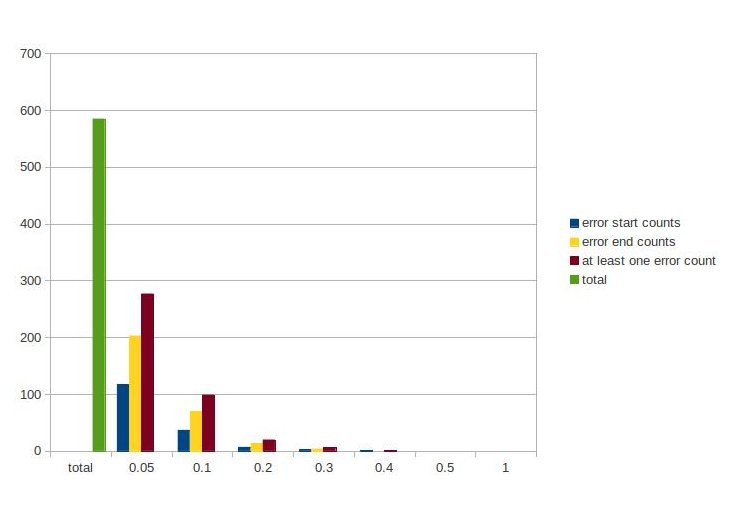
\includegraphics[scale=0.37]{doktor_piotr_length_based_counts.jpg}
    Dropping to 0 at 0.5 second difference, while getting to 99\% of correct tags for error of 300ms.
\end{frame}

\subsection{Results - “Boże Narodzenie”}
\begin{frame}
    \frametitle{Statistics - “Boże Narodzenie”}
    \begin{itemize}
        \item Total number of words				\textbf{1779}
        \item Maximum difference (start or end): 			\textbf{0.606s}
        \item Maximum difference (start or end), if label was to short at one end: 			\textbf{0.605s}
        \item Average difference  (start or end):			\textbf{0.046s}
    \end{itemize}
\end{frame}
\begin{frame}
    \frametitle{Error counts - “Boże Narodzenie”}
    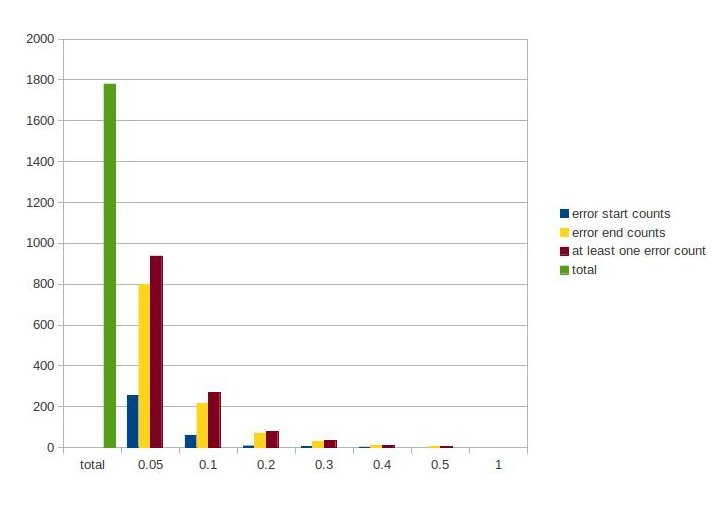
\includegraphics[scale=0.37]{boze_narodzenie_length_based_counts.jpg}
    Dropping to 0 at 1 second difference, while exceeding 98\% of correct tags for error of 300ms.
\end{frame}

\section{Synthesizer}
\subsection{Outline of algorithm}
\begin{frame}
    \frametitle{Input}
    \begin{itemize}
        \item audio recording
        \item phoneme alignment
        \item word alignment
        \item text to be synthesized
    \end{itemize}
\end{frame}
\begin{frame}
    \frametitle{Algorithm outline}
    \begin{itemize}
        \item for each word pick suitable candidates or synthesize one
        \item merge word candidates to create audio, as smoothly as possible
    \end{itemize}
\end{frame}
\begin{frame}
    \frametitle{Word synthesis}
    \begin{itemize}
        \item choose phoneme candidates (at least two at once)
        \item merge candidates so the total difference is minimized
        \item difference between two parts is a frame distance in best merging point
        \item best merging point candidates are in the middle of a phoneme
    \end{itemize}
\end{frame}
\begin{frame}
    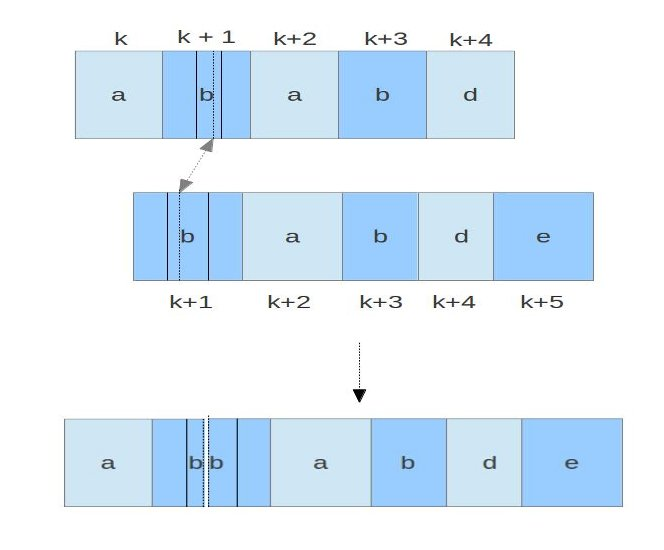
\includegraphics[scale=0.37]{audio_merging.jpg}
\end{frame}
\subsection{Results}
\begin{frame}
    \frametitle{Sample synthesized texts}
    \begin{itemize}
        \item<2-> "W czasie suszy szosa sucha"
        \item<3-> "Za górami za lasami znajduję się wysoka wieża strzeżona przez smoka"
        \item<4-> "Litwo Ojczyzno moja ty jesteś jak zdrowie Ile cię trzeba cenić ten tylko się dowie Kto cię stracił Dziś piękność twą w całej ozdobie Widzę i opisuję bo tęsknię po tobie"
        \item<5-> "Chrząszcz brzmi w trzcinie w Szczebrzeszynie W szczękach chrząszcza trzeszczy miąższ Czcza szczypawka czka w Szczecinie"
        \item<6-> "Rosja przedwojenna była wymarzoną areną dorobku dla ludzi tego typu zwłaszcza pochodzących z Królestwa"
    \end{itemize}
\end{frame}

\section{Conclusions}

\begin{frame}
    \frametitle{Conclusions}
    I believe that I managed to show in this thesis, that word alignment can be done without much apriori knowledge.
    My algorithm was able to return a decent alignment for an input audio file and recorded text with only knowledge about:
    \begin{enumerate}
        \item punctuation marks and their relationship to pauses
        \item a bit of knowledge about relationship between graphemes and phonemes (conversions grammars)
        \item a human anatomy and capabilities, especially about speech frequency ranges
        \item assumption that the input text has a high accuracy
    \end{enumerate}
\end{frame}

\end{document}

